%%%----------------------------------------------------------
\chapter{Still}
%%%----------------------------------------------------------

The activity "still" will be analyzed here with graphics.
%%%----------------------------------------------------------
\section{Test case 1}
%%%----------------------------------------------------------
Test case 1 in Fig.~\ref{fig:Test_case_still_1}
\begin{figure}
	\centering\small
	\setlength{\tabcolsep}{0mm}	% alle Spaltenränder auf 0mm
	\begin{tabular}{c@{\hspace{12mm}}c} % mittlerer Abstand = 12mm
		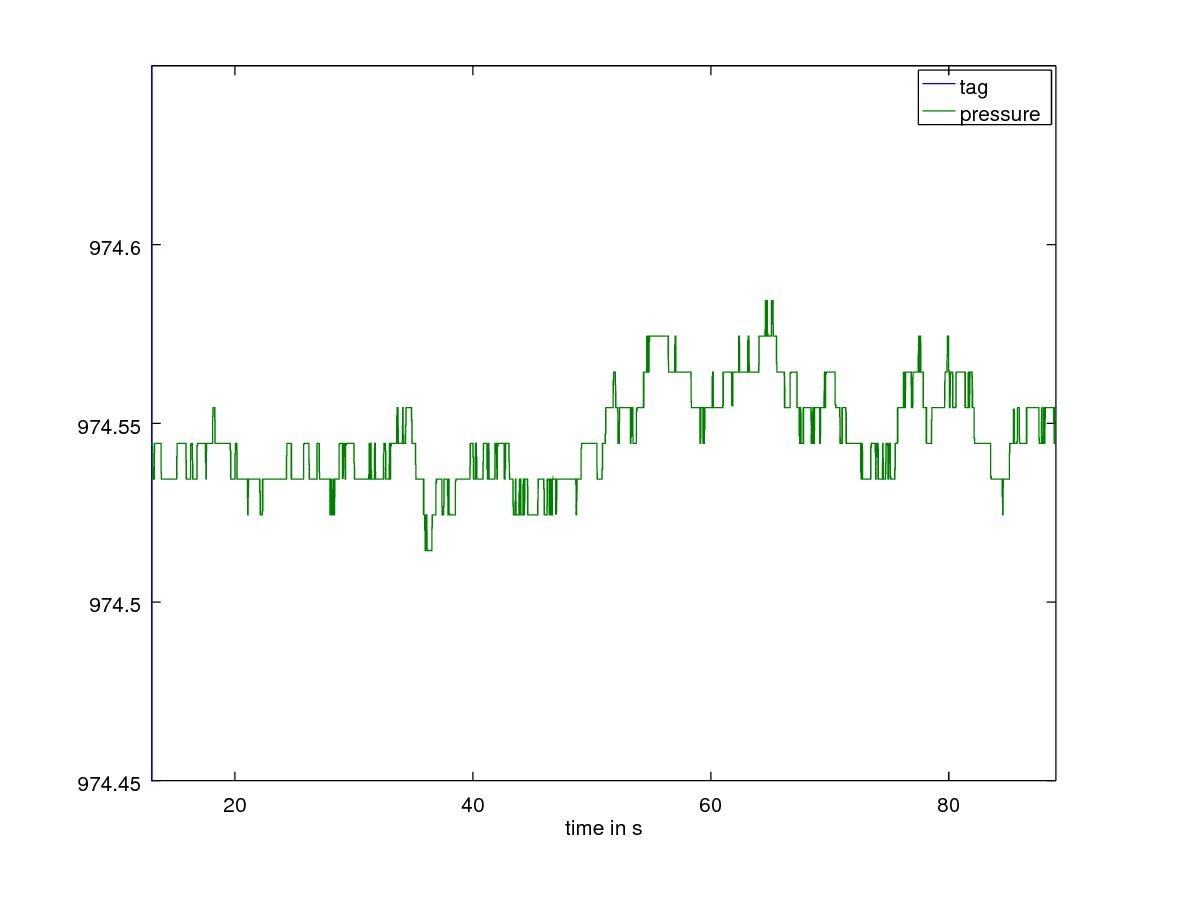
\includegraphics[width=.45\textwidth]{elevator4down1stop_still_p} &
		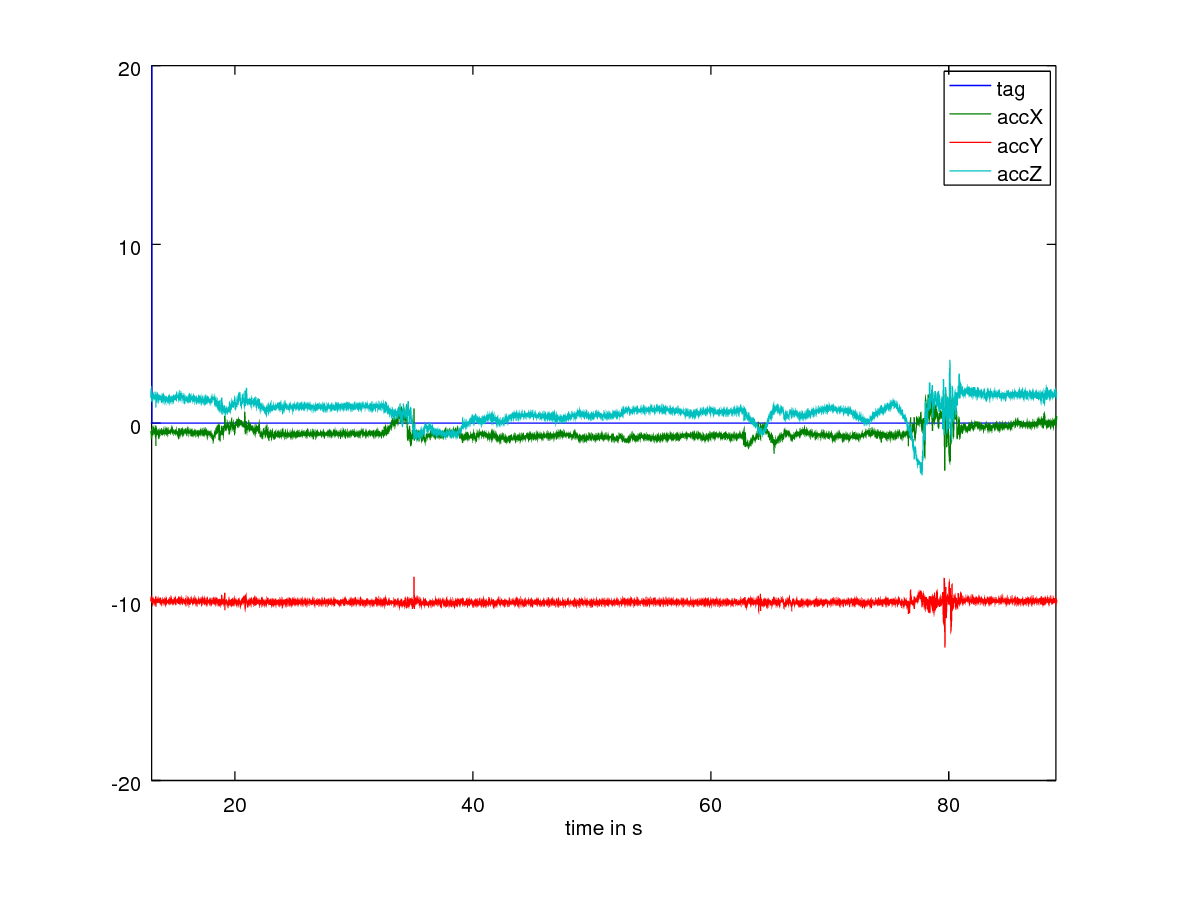
\includegraphics[width=.45\textwidth]{elevator4down1stop_still_a} 
		\\
		(a) & (b)
		\\[4pt]	%vertical extra spacing (4 points)
		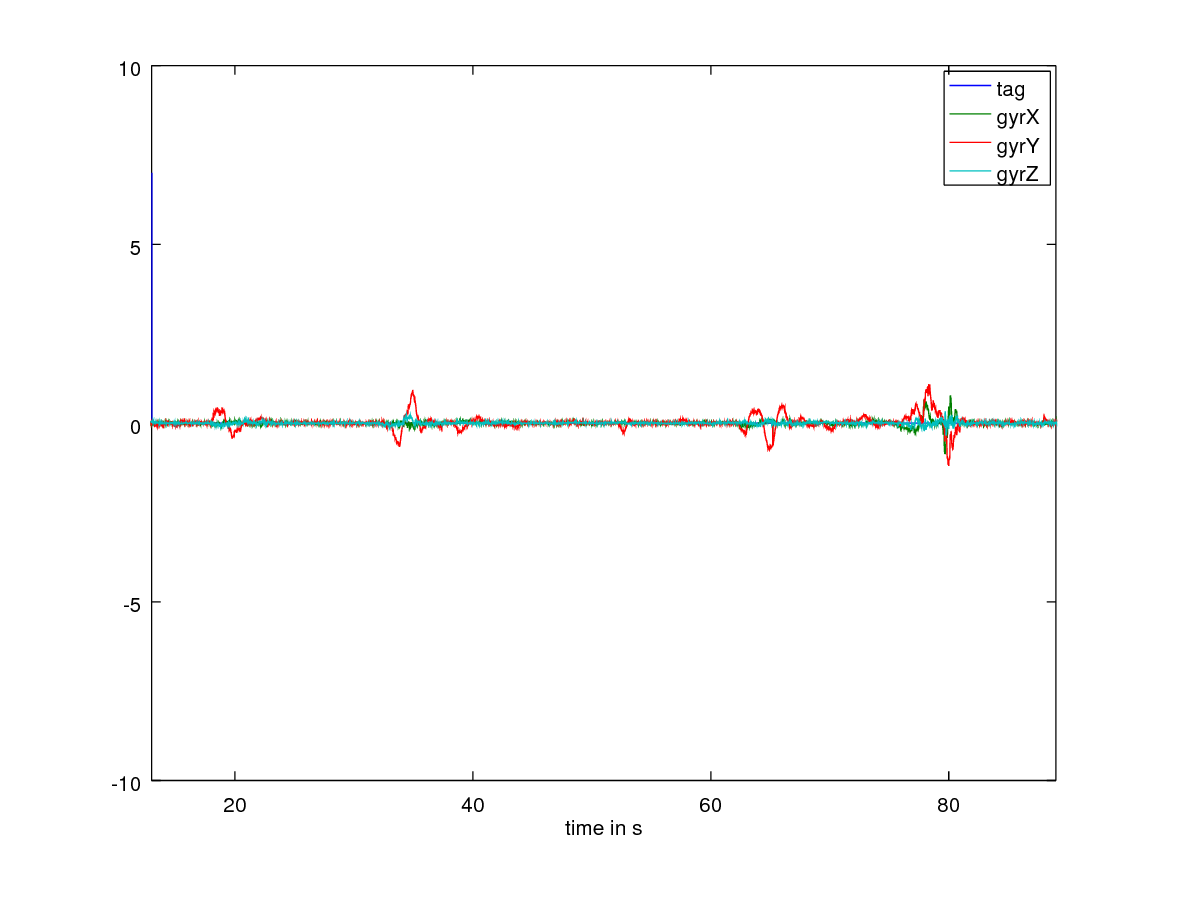
\includegraphics[width=.45\textwidth]{elevator4down1stop_still_g} &
		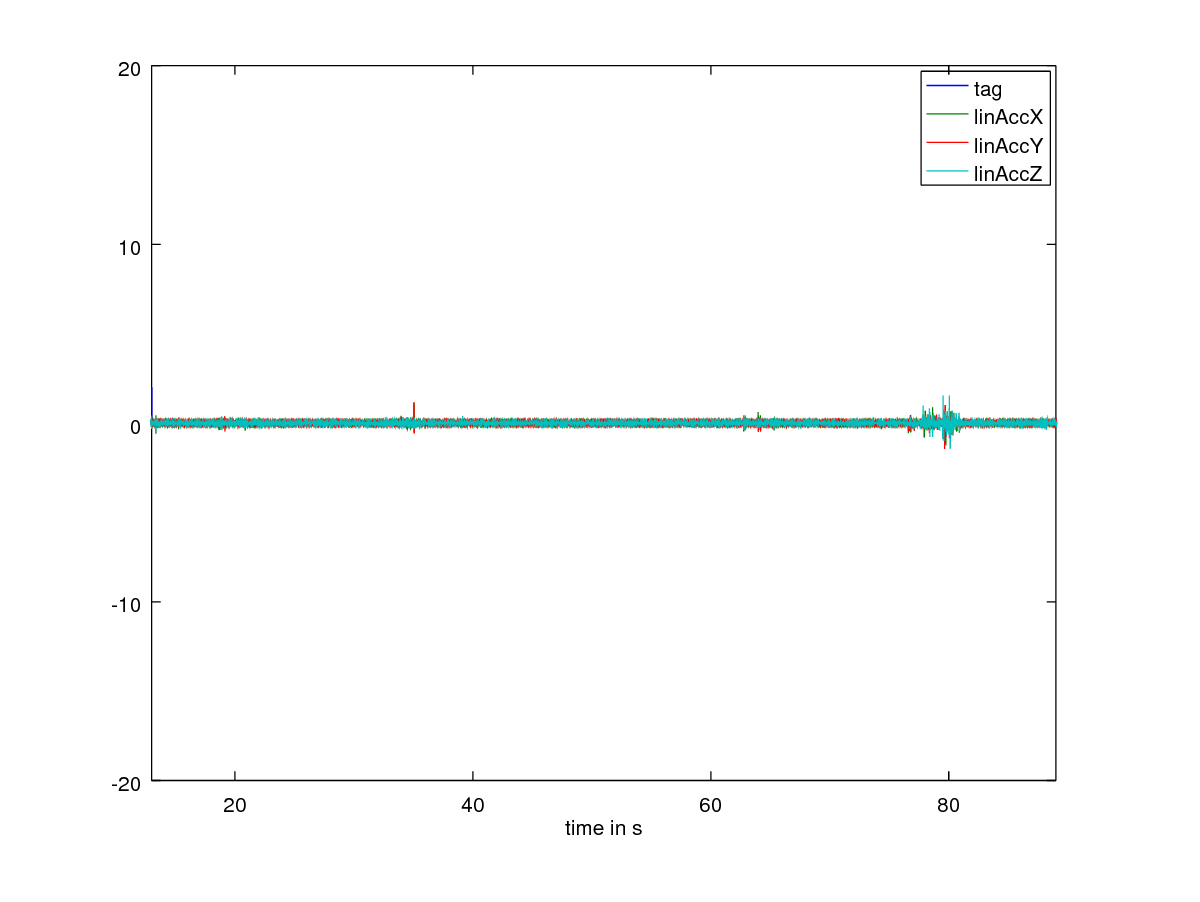
\includegraphics[width=.45\textwidth]{elevator4down1stop_still_la}
		\\
		(c) & (d)
		\\[4pt]	%vertical extra spacing (4 points)
		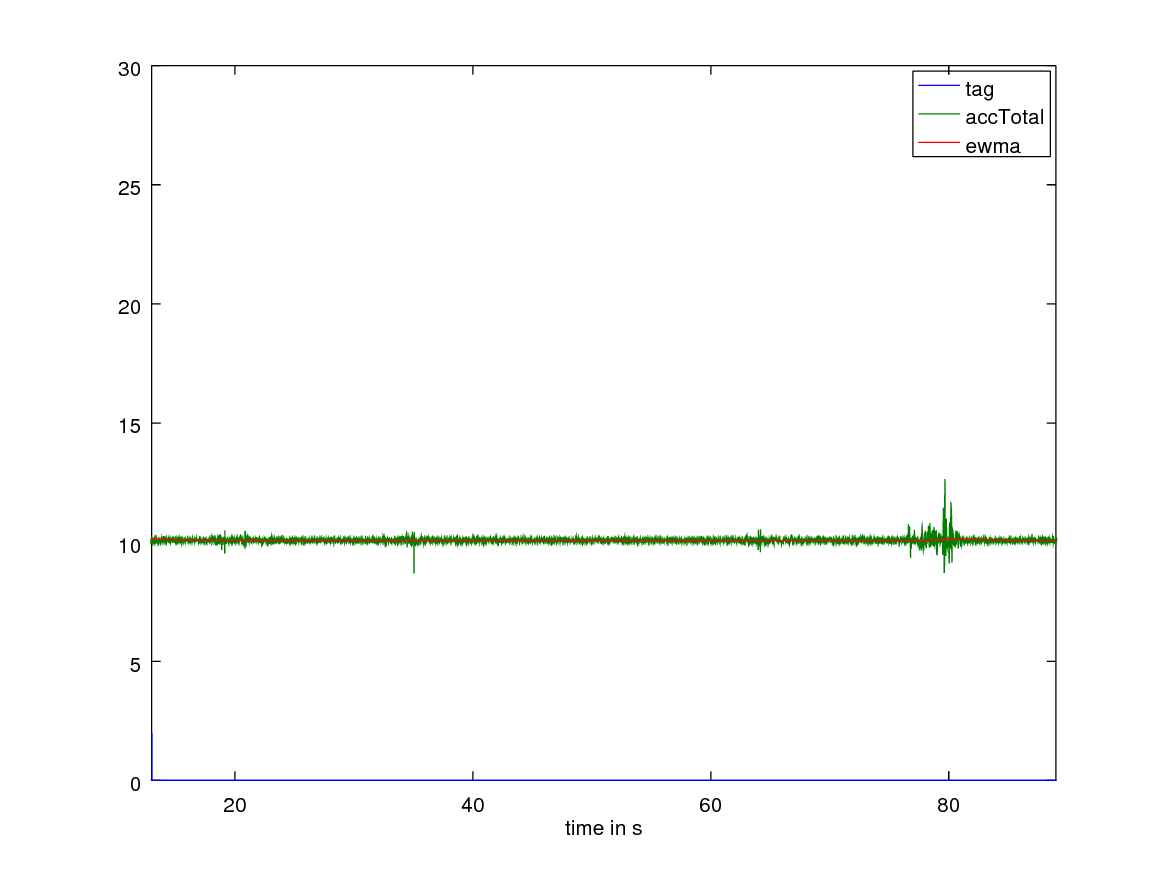
\includegraphics[width=.45\textwidth]{elevator4down1stop_still_atotal} &
		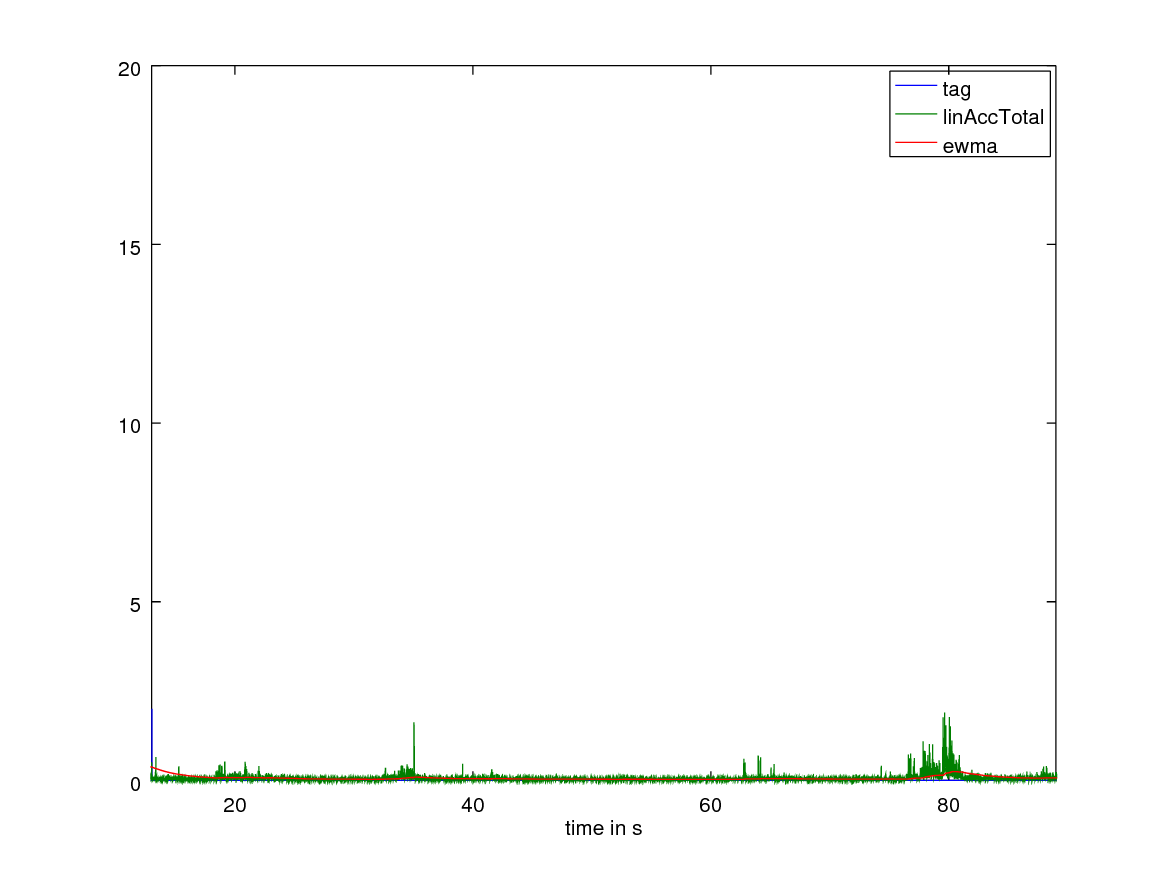
\includegraphics[width=.45\textwidth]{elevator4down1stop_still_latotal}
		\\
		(e) & (f)
	\end{tabular}
	%
	\caption{Test case 1}
	\label{fig:Test_case_still_1}
\end{figure}

%%%----------------------------------------------------------
\section{Test case 2}
%%%----------------------------------------------------------
Test case 2 in Fig.~\ref{fig:Test_case_still_2}
\begin{figure}
	\centering\small
	\setlength{\tabcolsep}{0mm}	% alle Spaltenränder auf 0mm
	\begin{tabular}{c@{\hspace{12mm}}c} % mittlerer Abstand = 12mm
		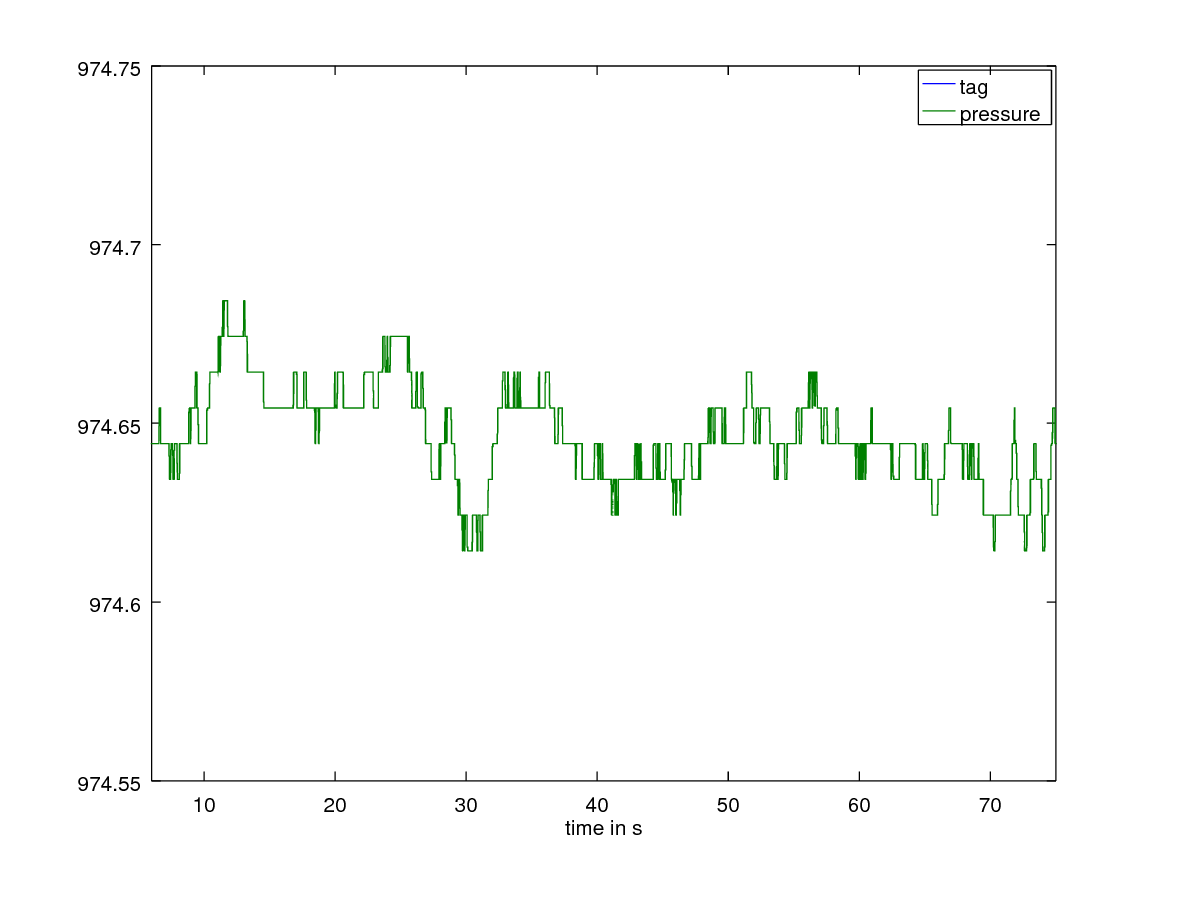
\includegraphics[width=.45\textwidth]{elevator4down2stops_still_p} &
		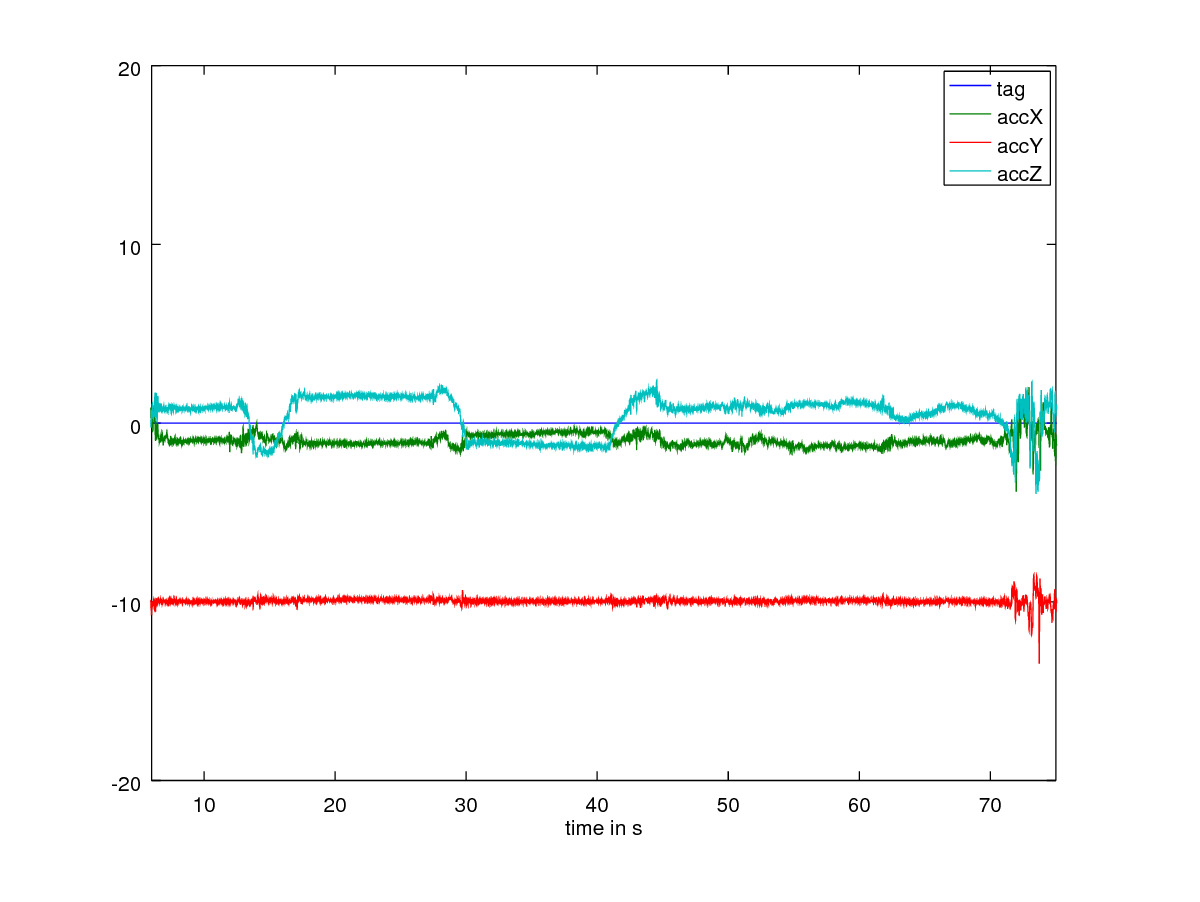
\includegraphics[width=.45\textwidth]{elevator4down2stops_still_a} 
		\\
		(a) & (b)
		\\[4pt]	%vertical extra spacing (4 points)
		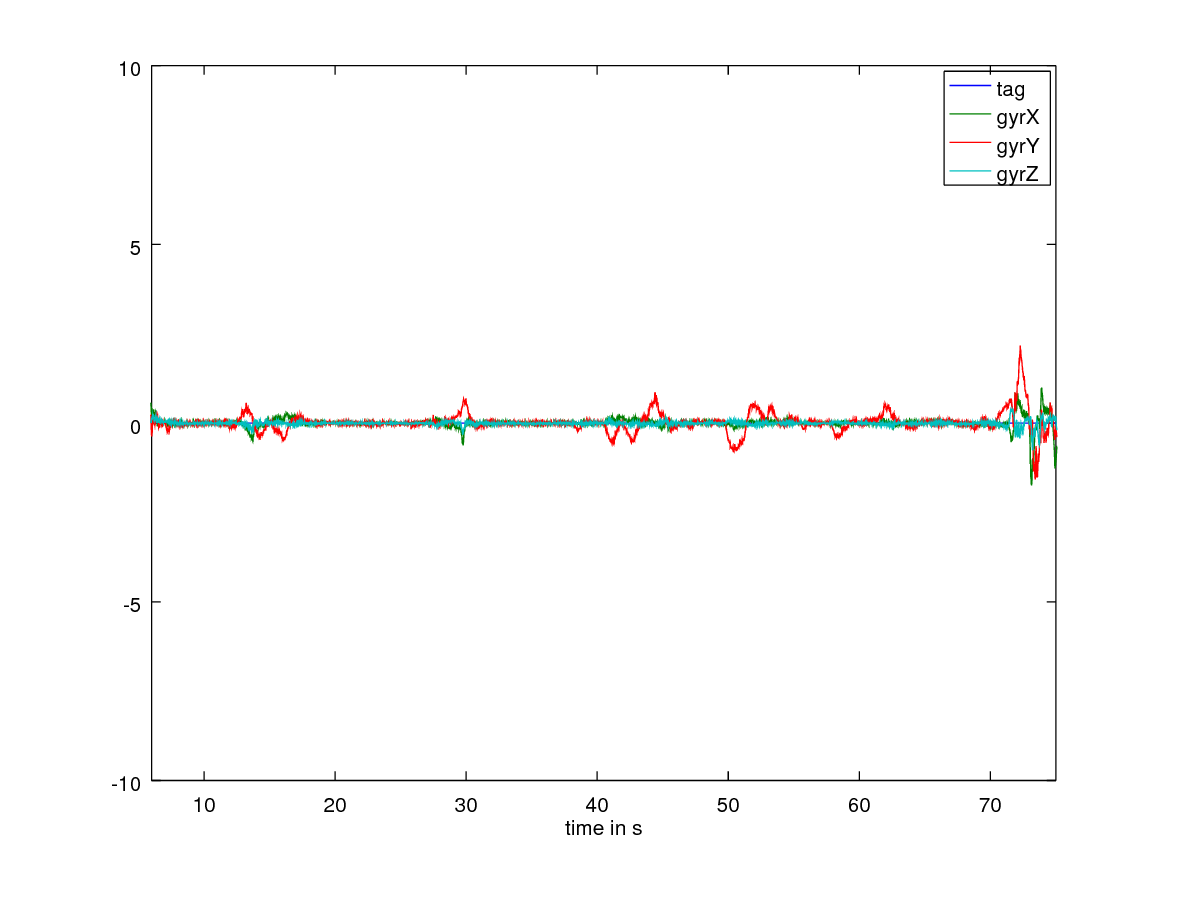
\includegraphics[width=.45\textwidth]{elevator4down2stops_still_g} &
		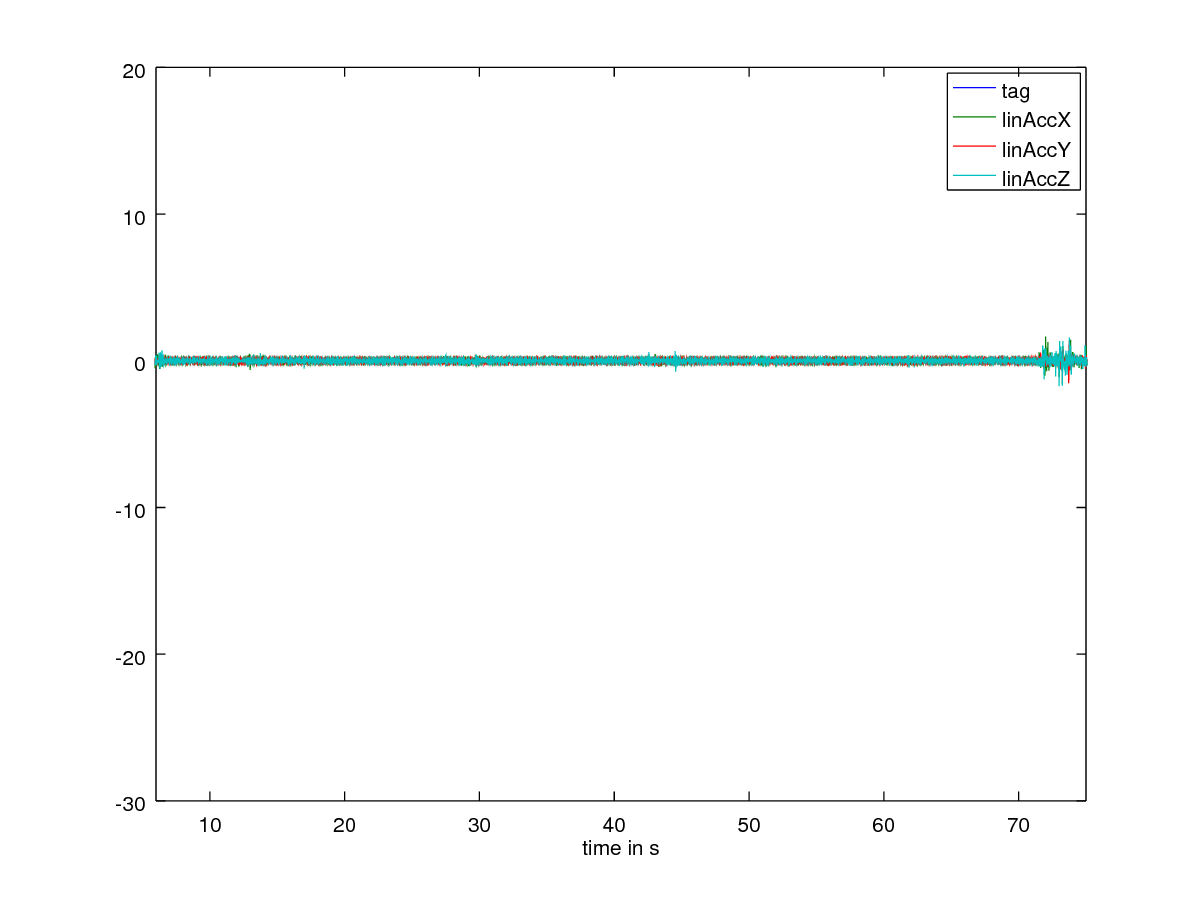
\includegraphics[width=.45\textwidth]{elevator4down2stops_still_la}
		\\
		(c) & (d)
		\\[4pt]	%vertical extra spacing (4 points)
		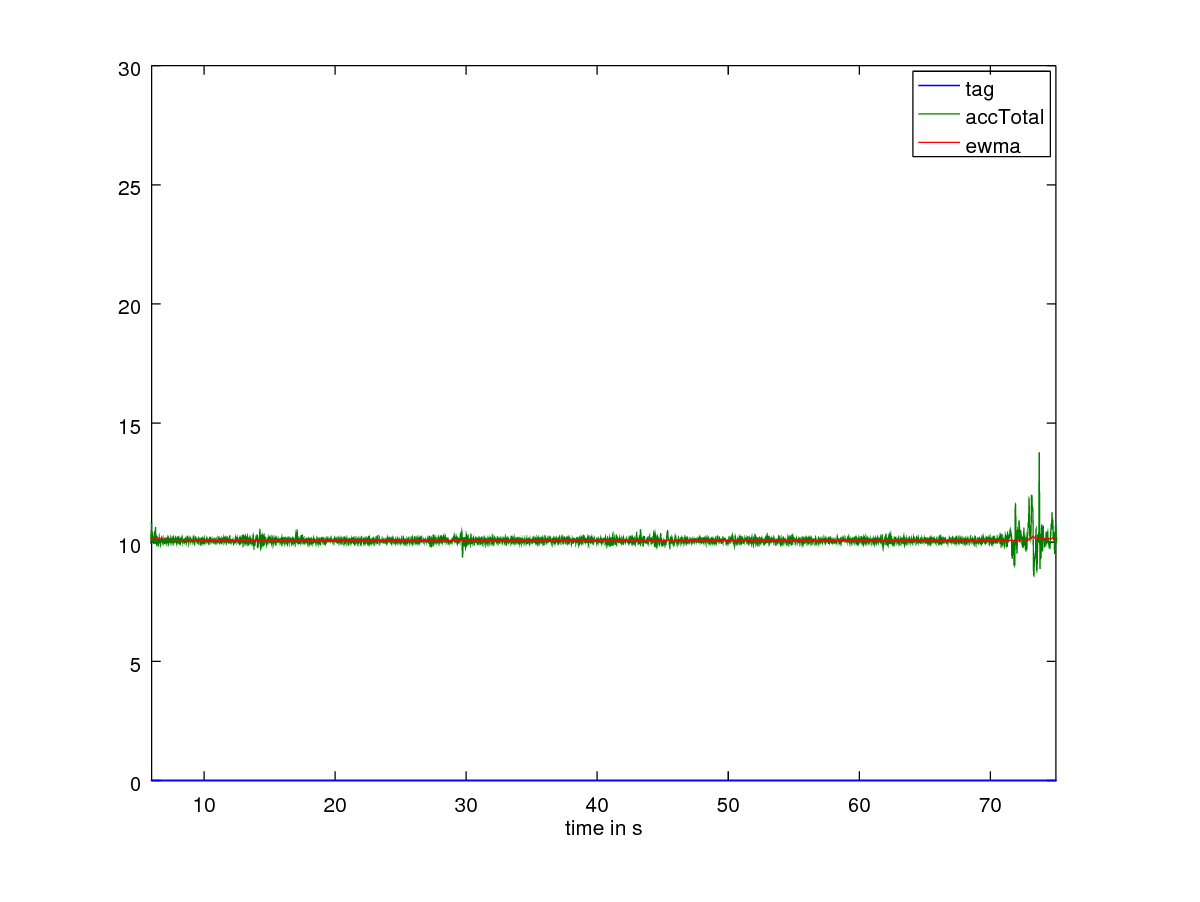
\includegraphics[width=.45\textwidth]{elevator4down2stops_still_atotal} &
		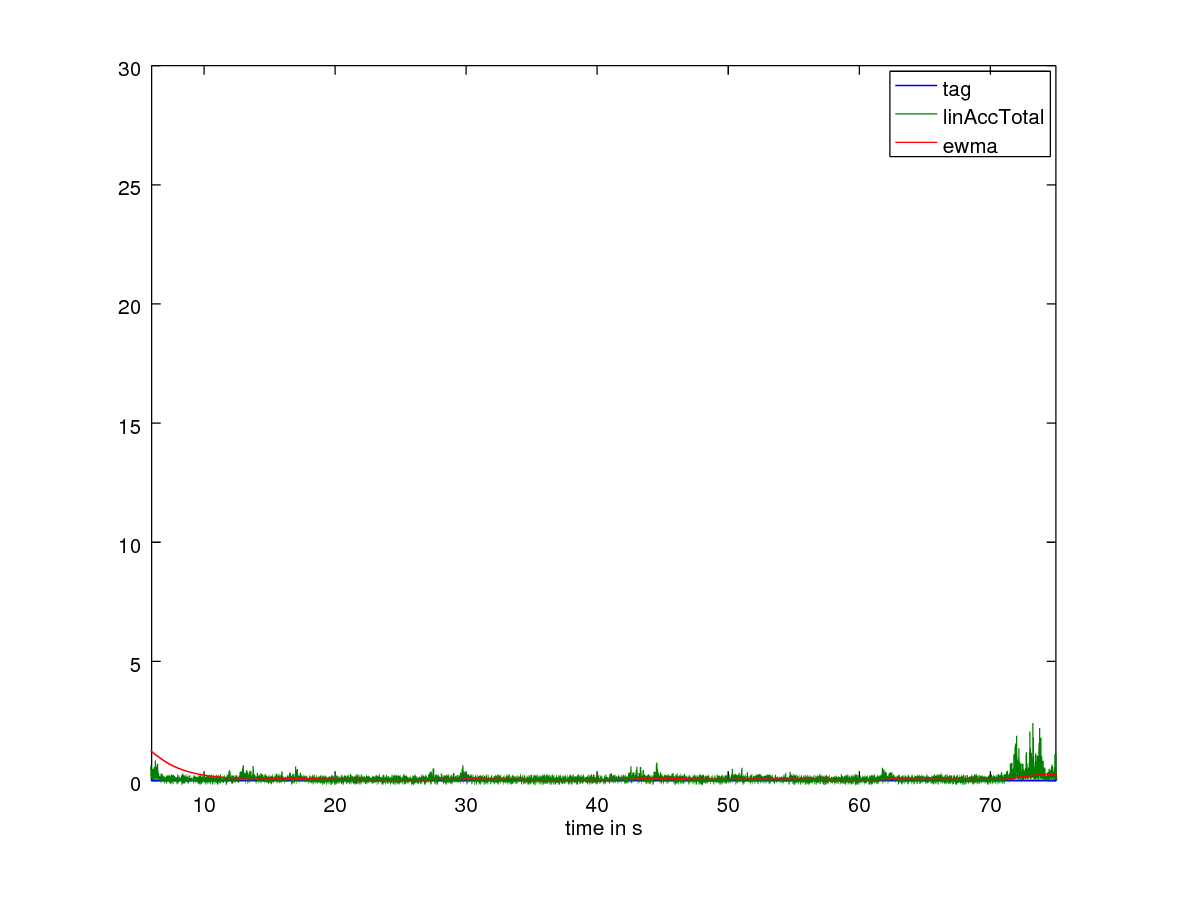
\includegraphics[width=.45\textwidth]{elevator4down2stops_still_latotal}
		\\
		(e) & (f)
	\end{tabular}
	%
	\caption{Test case 2}
	\label{fig:Test_case_still_2}
\end{figure}

%%%----------------------------------------------------------
\section{Test case 3}
%%%----------------------------------------------------------
Test case 3 in Fig.~\ref{fig:Test_case_still_3}
\begin{figure}
	\centering\small
	\setlength{\tabcolsep}{0mm}	% alle Spaltenränder auf 0mm
	\begin{tabular}{c@{\hspace{12mm}}c} % mittlerer Abstand = 12mm
			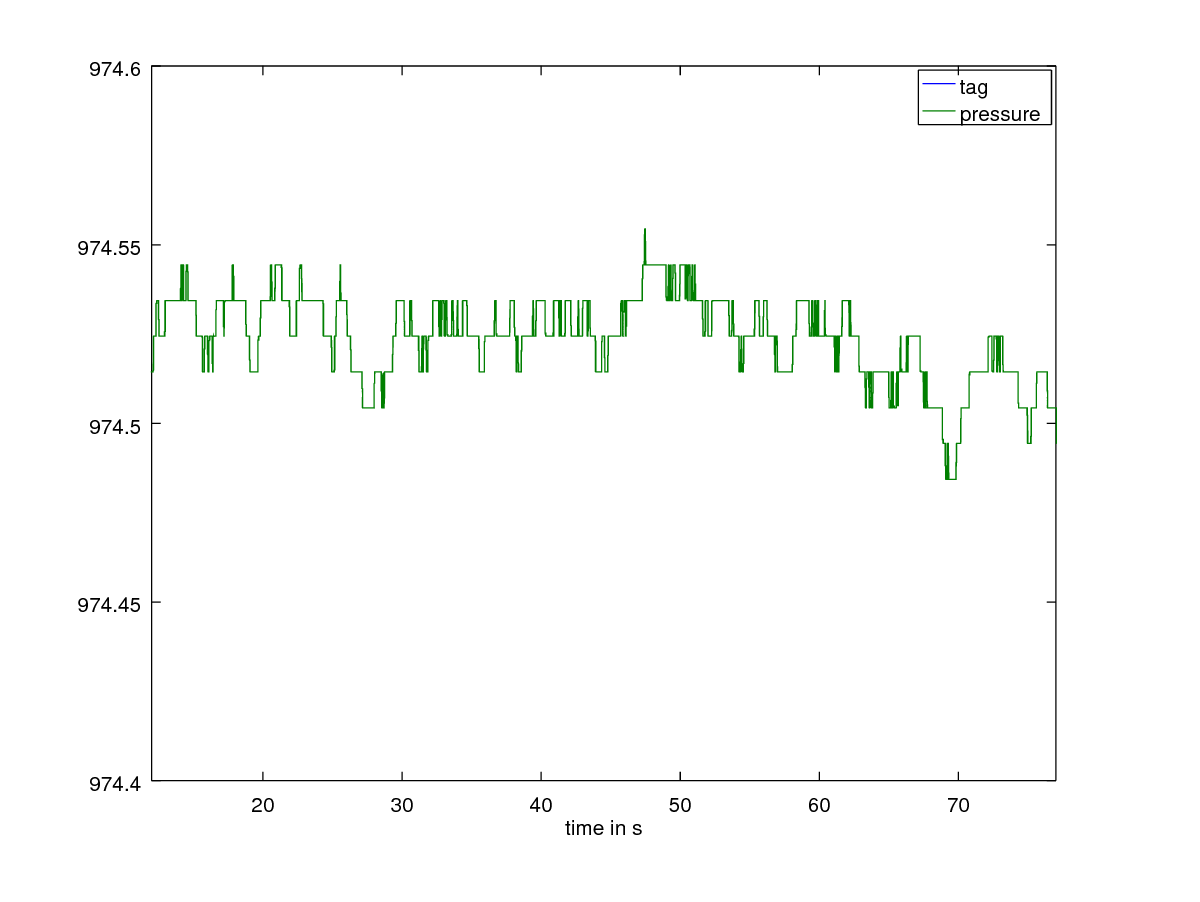
\includegraphics[width=.45\textwidth]{elevator5down1stop_still_p} &
			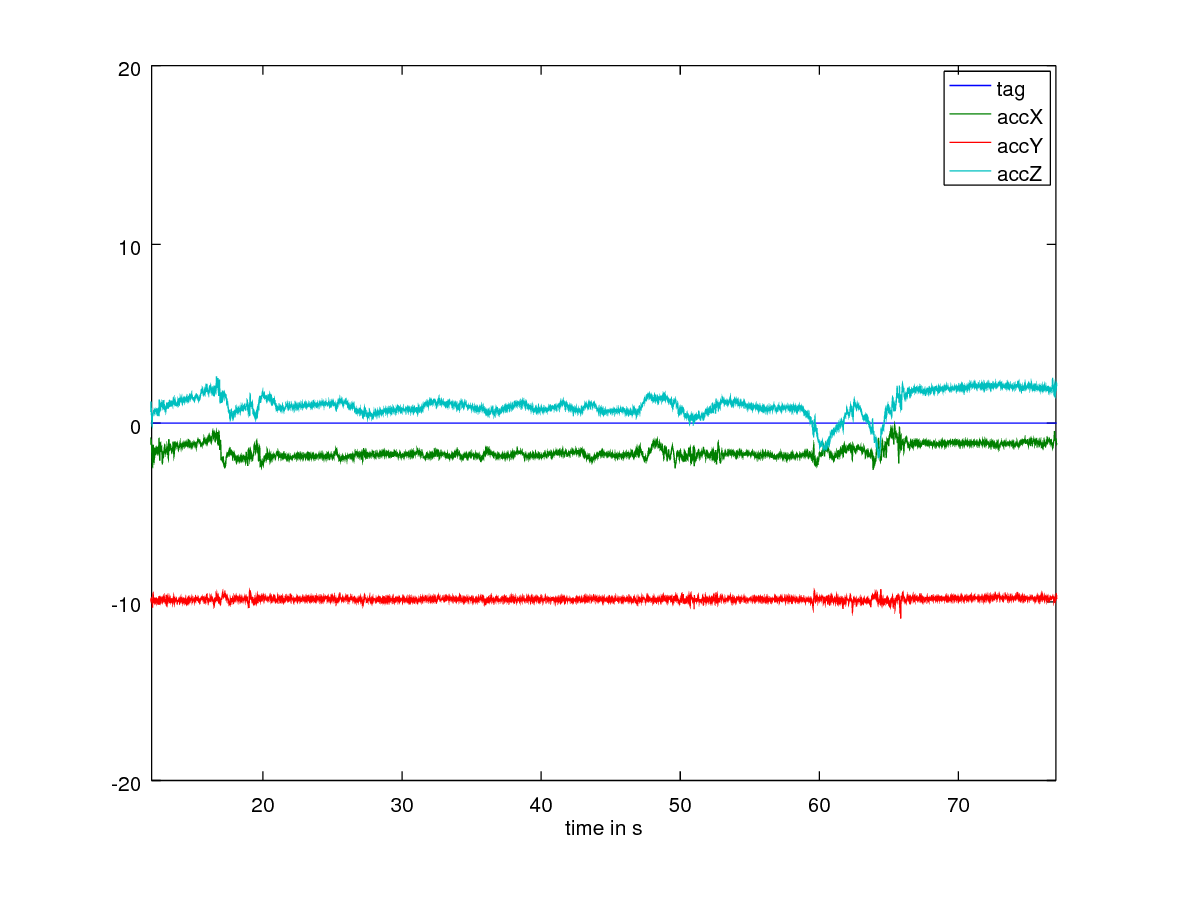
\includegraphics[width=.45\textwidth]{elevator5down1stop_still_a} 
			\\
			(a) & (b)
			\\[4pt]	%vertical extra spacing (4 points)
			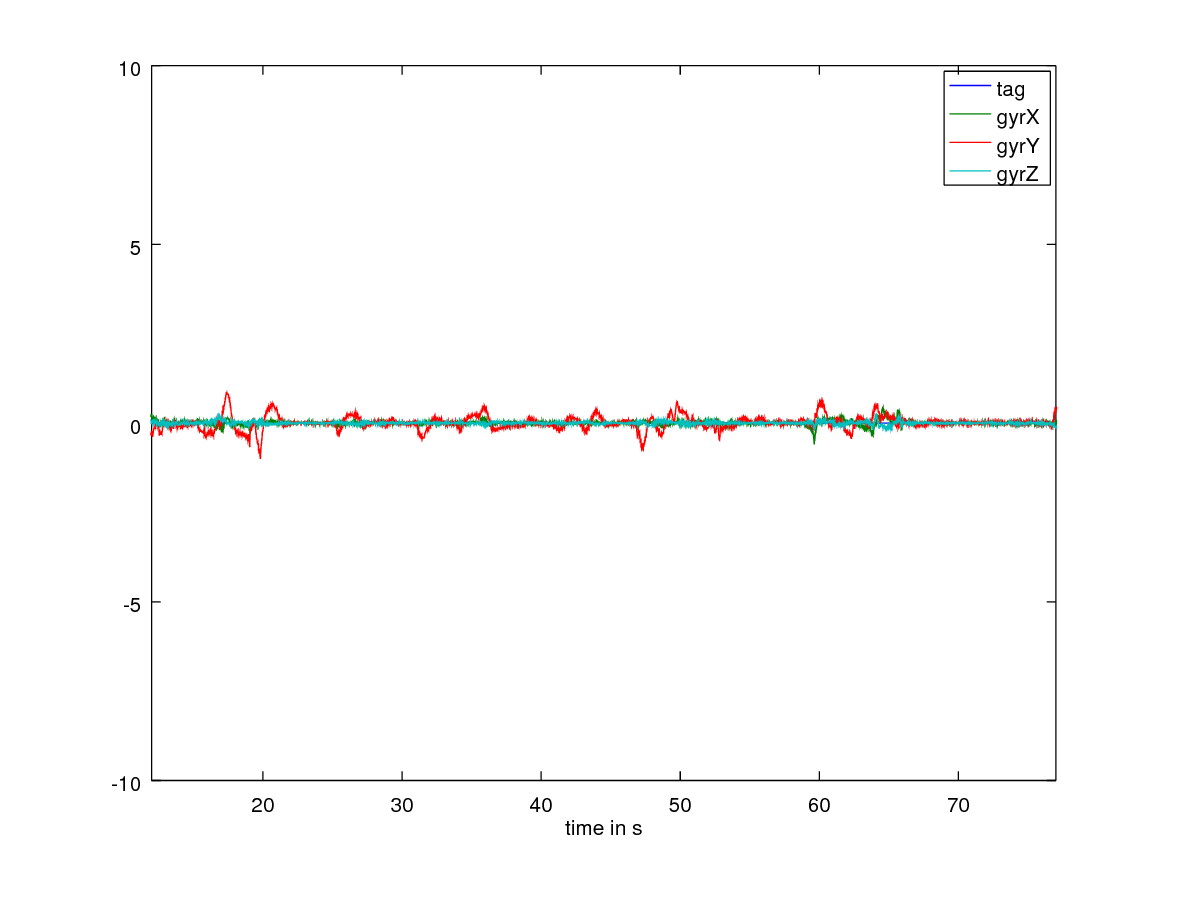
\includegraphics[width=.45\textwidth]{elevator5down1stop_still_g} &
			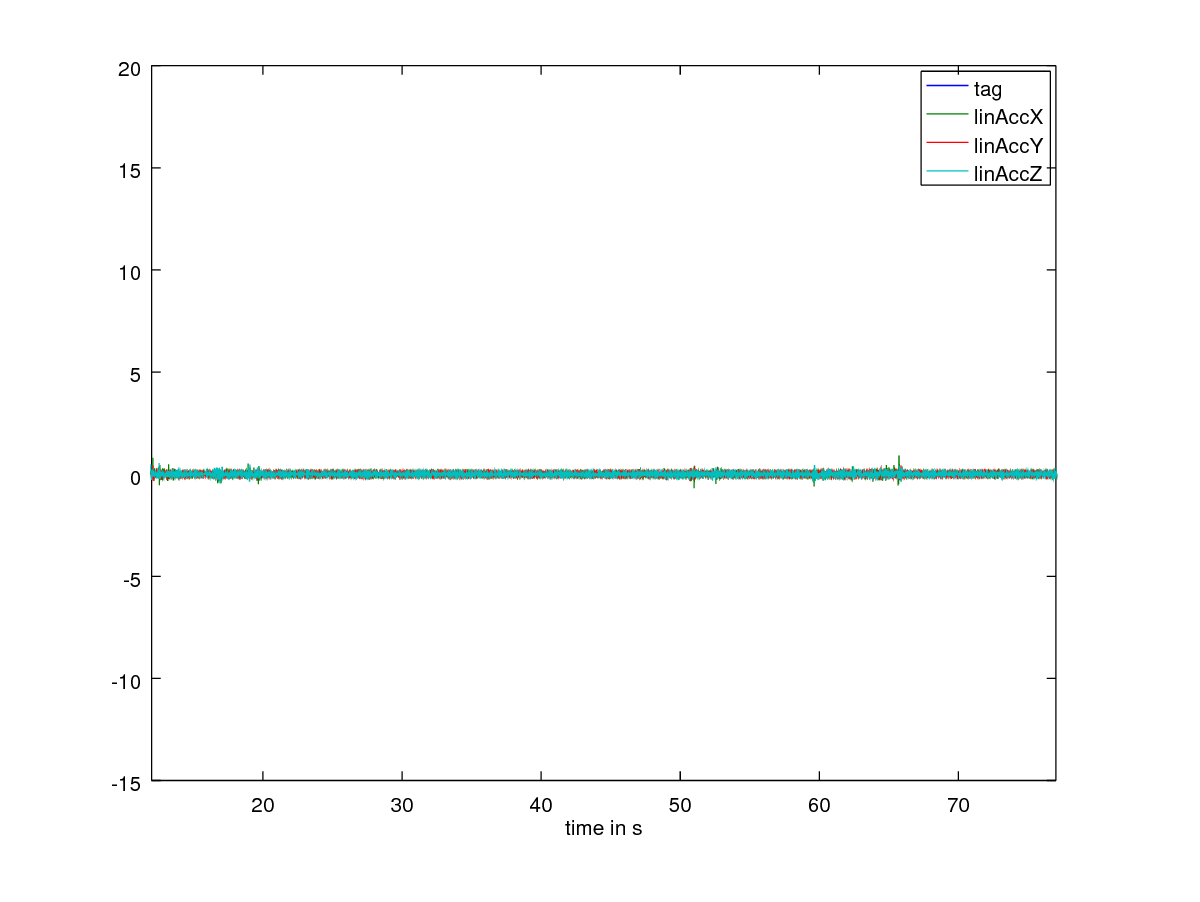
\includegraphics[width=.45\textwidth]{elevator5down1stop_still_la}
			\\
			(c) & (d)
			\\[4pt]	%vertical extra spacing (4 points)
			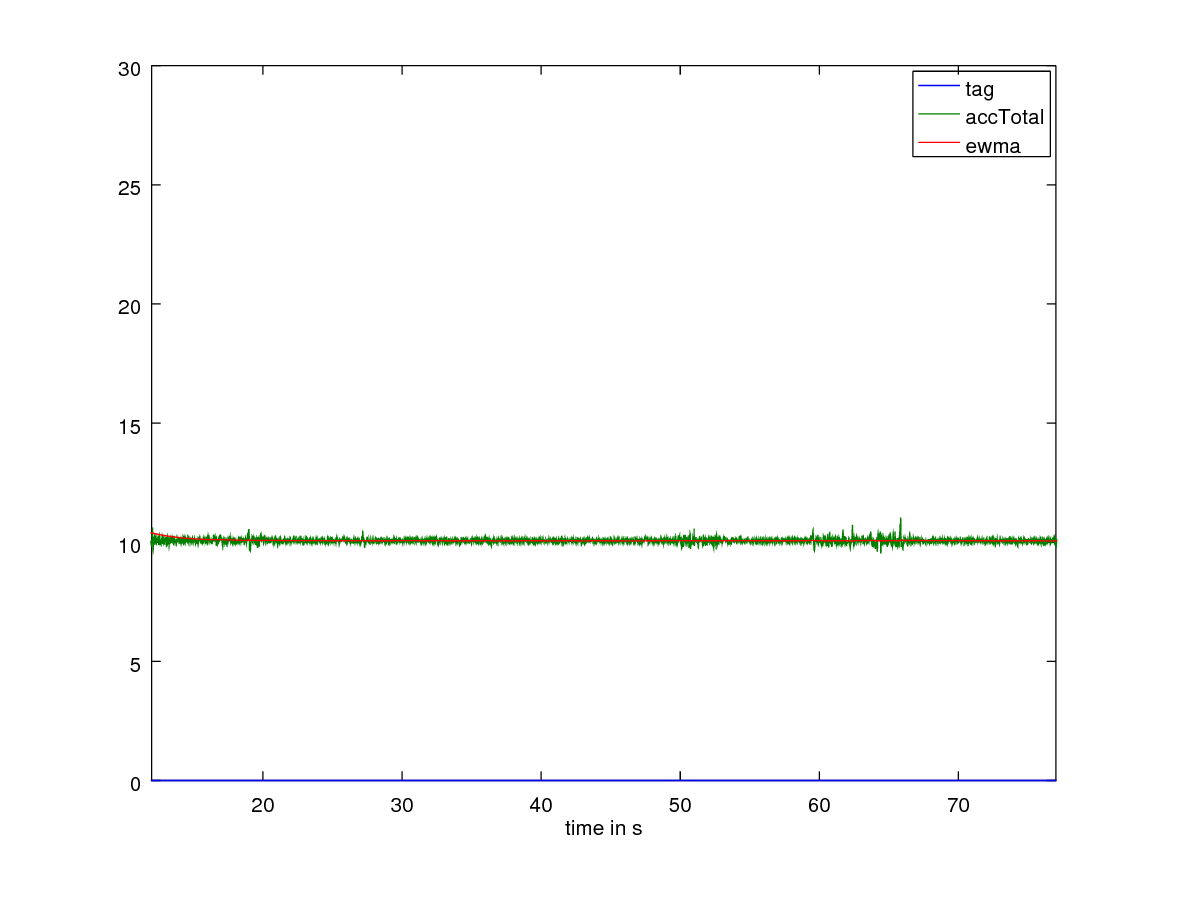
\includegraphics[width=.45\textwidth]{elevator5down1stop_still_atotal} &
			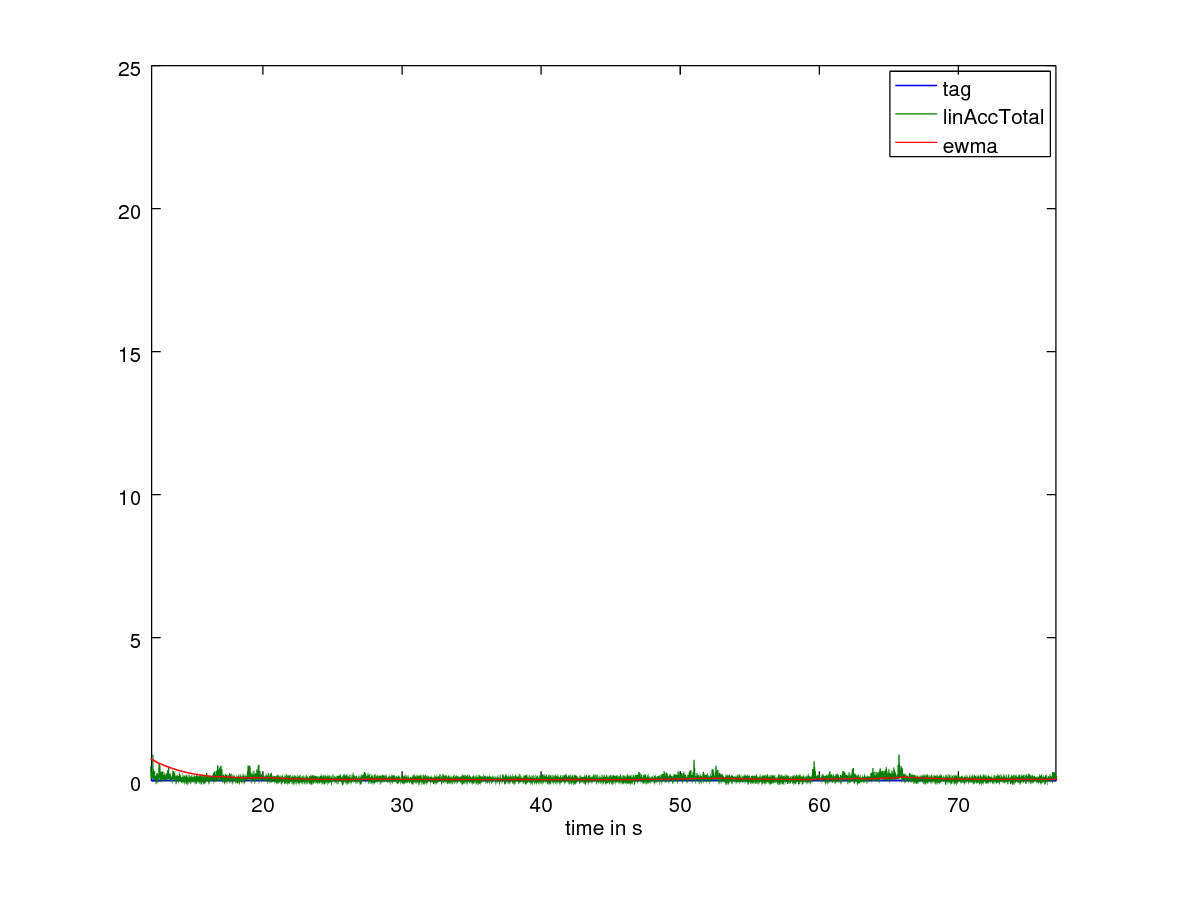
\includegraphics[width=.45\textwidth]{elevator5down1stop_still_latotal}
			\\
			(e) & (f)
	\end{tabular}
	%
	\caption{Test case 3}
	\label{fig:Test_case_still_3}
\end{figure}

